\subsection{System architecture}
\begin{figure}[h]
    \centering
    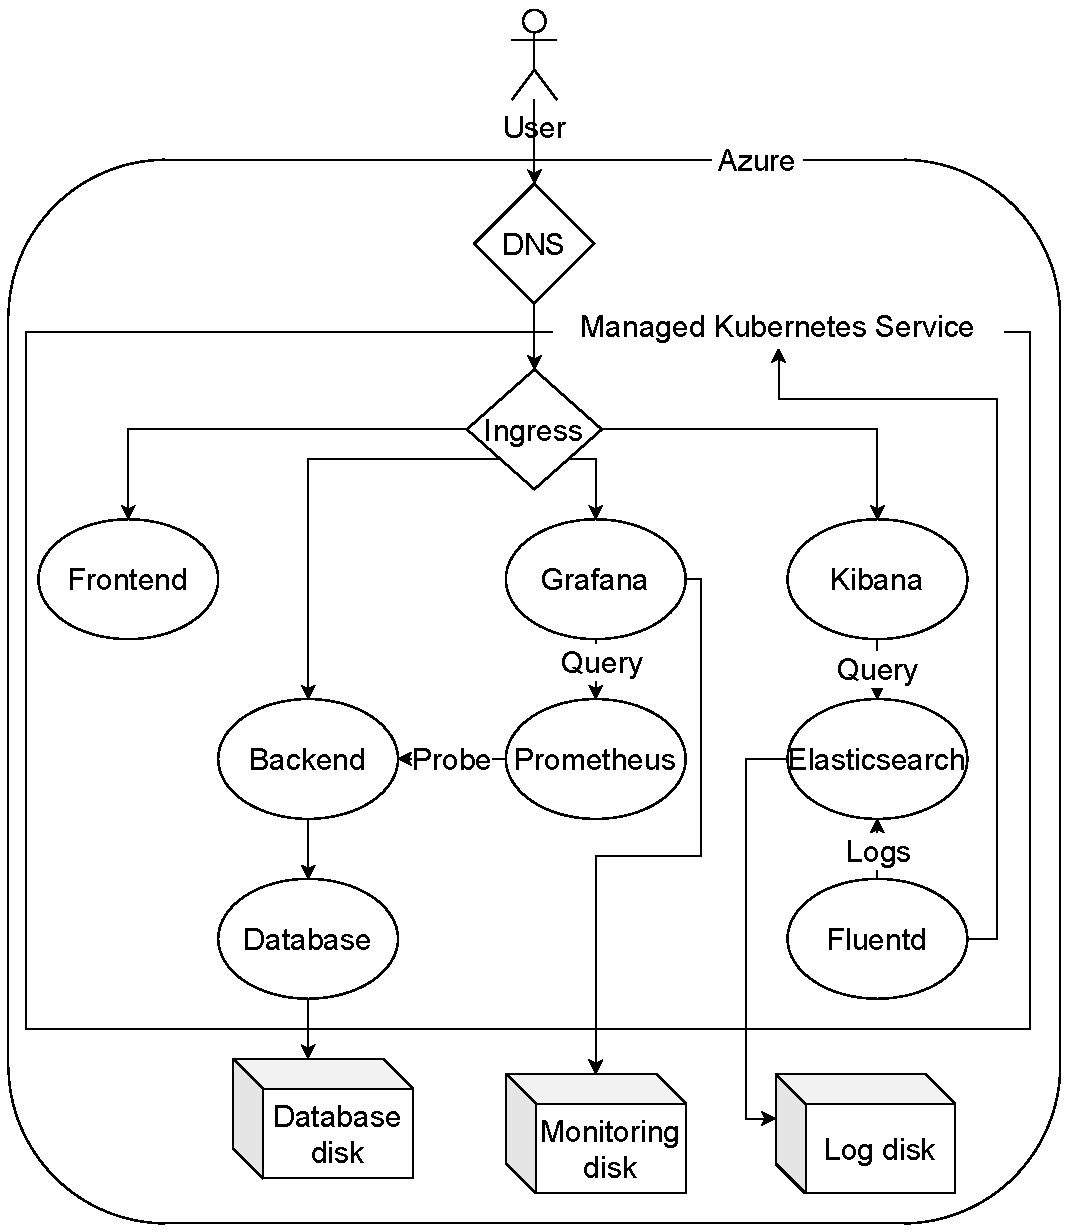
\includegraphics[width=0.8\textwidth]{infrastructure/infrastructure.pdf}
    \caption{System architecture and it's components}
    \label{fig:architecture}
\end{figure}

We've built our system twice, according to 2 specifications. The first was a, mostly, one to one rewrite of the original project into Go \cite{tool:go}.
While the second, and current iteration, was according to the API specification \cite{spec:api}. 
This iteration consists of 4 subsystems and supporting infrastructure. The subsystems we'll go through below are: backend, frontend, monitoring and logging.
The overview and interaction between these systems are modelled in figure \ref{fig:architecture}.

\subsubsection{Backend}
The core system of the project is the backend. It is responsible for the actual computations and controlling of the database.
It's built with Go \cite{tool:go}, runs in a Docker container and uses Microsoft SQL server \cite{tool:microsoft-sql-server} as the database. We deep dive into this component in the "System Design" section - section \ref{section:system-design}.

\subsubsection{Frontend}
As the backend changed from server rendered website to a REST API, we decided to move the frontend into it's own subsystem.
The frontend is built with Vue.js \cite{tool:vue} and is written in TypeScript \cite{tool:typescript}.
It makes use of the public API that the backend exposes, and therefore provides a more user friendly access layer to our service.
The subsystem is built in small components that can be reused when expanding the project. We had a focus on the visual elements being mostly identical to the original frontend, to ensure user familiarity.

\subsubsection{Monitoring}
To keep track of the health of our system, its performance, usage and other metrics, we use Prometheus \cite{tool:prometheus} to collect metrics and Grafana \cite{tool:grafana} to view said metrics.
Our metrics include: CPU usage, memory usage, number of requests per endpoint, average request latency and amount of registered users.
These metrics provide an overview over the system health and allows us to diagnose issues faster, by locating when something happened, at which endpoint and if it had an effect on system resources.

\subsubsection{Logging}
For more detailed diagnostics we have a logging subsystem. It's built with Fluentd \cite{tool:fluentd}, Elasticsearch \cite{tool:elasticsearch}, and Kibana \cite{tool:kibana}.
Fluentd reads the logs from the Kubernetes host, and parses them according to the configured log format.
It then tags them and sends them to Elasticsearch, which indexes and stores them, such that they are easily searchable.
Kibana provides a web interface to search, read and display the logs in a structured way.\\

Having this logging system allows us to diagnose what happened when something goes wrong, as we can easily find and read the info, warnings and errors that our system outputs.

\subsubsection{Kubernetes and Azure}
To deploy this system we use Kubernetes \cite{tool:kubernetes} deployed on Azure \cite{tool:azure} through AKS \cite{tool:aks}.

Using Kubernetes makes us host agnostic.
A few times during the project we've had to move our host, which we've done without issue due to the emphasis on containerization and host abstraction that Kubernetes has.
Kubernetes also allows us to easily scale our system, as we can easily deploy new nodes and load balance our services.

We've used Azure as our deployment target, as it was reliable, familiar and cheap. AKS is Azure's managed Kubernetes service.

\subsubsection{Supporting infrastructure}
To make this infrastructure function we have some supporting infrastructure.
Such as our domain registrant where we bought our domain - one.com \cite{onecom}.
Our domain administrator that controls our domain and handles nameserver changes - DK Hostmaster \cite{dk-hostmaster}.
And our Azure hosted DNS zone \cite{tool:dns-zone} that handles dns records. This informs systems to route traffic to the correct infrastructure.
